\section{Chapter 5 - Problem (10)}

	The floor of a railroad flatcar is loaded with loose crates having a coefficient of static friction of $0.56$ with the floor. If the train is initially moving at a speed of $47 \ mi/h$, in how short a distance can the train be stopped at constant acceleration without causing the crates to slide over the floor?

	\textbf{R:} \newline

	\begin{figure}[H]
		\begin{center}
			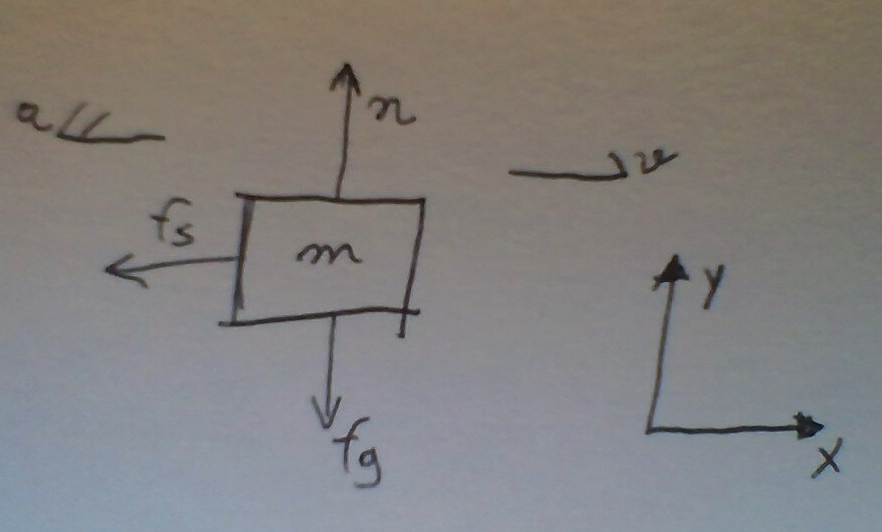
\includegraphics[scale=0.3]{hw6_problema_fbd}
			\caption{Free-Body Diagram (Problem 10)}
			\label{fig:hw6_problema_fbd}
		\end{center}
	\end{figure}

	Newton's $2^{nd}$ Law:
	\begin{align}
		\sum F_{y} = \ &ma_{y}& \notag \\
		n - mg = \ &m(0)& \notag \\
		n = \ &mg& \notag \\
		\sum F_{x} = \ &ma_{x}& \notag \\
		-f_{s} = \ &m(-a)& \notag \\
		f_{s} = \ &f_{s_{max}}& \notag \\
		ma = \ &\mu_{s}mg& \notag \\
		a = \ &\mu_{s}g& \notag \\
		a = \ &(0.56) \left( 32.2 \ ft/s^{2} \right)& \notag \\
		a = \ &18.032 ft/s^{2}& \notag
	\end{align}

	\begin{align}
		a = \ &-18.032 \ ft/s^{2}& \notag \\
		x_{0} = \ &0& \notag \\
		v_{0} = \ &47 \ mi/h
		\times \left( \frac{5280 \ ft}{1 \ mi} \right)
		\times \left( \frac{1 \ h}{3600 \ s} \right) = 68.9\bar{3} \ ft/s& \notag \\
		v = \ &0& \notag \\
		2a(x-x_{0}) = \ &v^{2} - v_{0}^{2}& \notag \\
		2\left( -18.032 ft/s^{2} \right)(x-0) = \ &(0)^{2} - (68.9\bar{3} \ ft/s)^{2}& \notag \\
		\left( -36.064 \ ft/s^{2} \right)x = \ &-4751.3449 \ ft^{2}/s^{2}& \notag \\
		x = \ &\frac{-4751.3449 \ ft^{2}/s^{2}}{-36.064 \ ft/s^{2}} = 131.8 \ ft&
	\end{align}
